

Figures \ref{overview} show the general overview of ParLOT's workflow.

\subsection{Tracing Operation}

\parlot is built on top of \pin. In particular, it instructs \pin to instrument every thread launch and termination in the application as well as every function entry and exit. The thread-launch instrumentation code initializes the per-thread tracing variables and opens a file into which the trace data from that thread will be written. The thread-termination code finalizes any ongoing compression, flushes out the remaining buffer entries, and closes the trace file. \parlot assigns every static function in each image (main program and all libraries) a unique unsigned 16-bit ID, which it records in a separate file together with the image and function name. This file later serves to map IDs back to image/function-name pairs.

For every function \emph{entry}, \parlot executes extra code that has access to the thread ID, function ID, and current stack-pointer (SP) value. Based on the SP value, it performs call-stack correction if necessary (see below), adds the new function to a data structure it maintains that holds the call stack (which is different from the application’s runtime stack), and emits the function ID into the trace file via an incremental compression algorithm (see below). All of this is done independently for each thread. Similarly, for every function \emph{exit}, \parlot also executes extra code that has access to the thread ID, function ID, and current SP value. Based on the SP value, it performs call-stack correction if necessary, removes the function from its call-stack data structure, and emits the reserved function ID value of zero into the trace file to indicate an exit. As before, this is done via an incremental compression algorithm. We use zero for all exits rather than emitting the function ID and a bit to specify whether it is an entry or exit because using zeros results in more compressible output. After all, this way, half of the values in the trace will be zero.

\subsection{Call-Stack Correction}

To be able to decode the trace, i.e., to correctly associate each exit with the function entry it belongs to, our trace reader maintains an identical call-stack data structure. Unfortunately, and as pointed out in the \pin documentation, it is not always possible to identify all function exits. For example, in highly optimized code, a function’s instructions may be inlined and interleaved with the caller’s instructions, making it infeasible for \pin to identify the exit. As a consequence, \parlot has to work correctly even when \pin occasionally misses an exit. This is where the SP values come into play.

During tracing, \parlot not only records the function IDs in its call-stack data structure but also the associated SP values. This enables it to detect missing exits and to correct the call stack accordingly. Whenever a function is entered, it checks if there is at least one entry in the call stack and, if so, whether its SP value is higher than that of the current SP. If it is lower, we must have missed at least one exit since the runtime stack grows downwards and, therefore, the SP value decreases with every function entry and increases with every exit. If a missing exit is detected in this manner, \parlot pops the top element from its call stack and emits a zero to indicate a function exit. It repeats this procedure until the stack is empty or its top entry has a sufficiently high SP value. The same call-stack correction technique is applied for every function exit whose SP value is inconsistent. Note that the SP values are only used for this purpose and are not included in the emitted trace data.

The result is an internally consistent trace of function entry and exit events, meaning that parsing the trace will yield a correct call stack. This is essential so that the trace can be decoded correctly. Moreover, it means that the trace includes exits that truly happened in the application but that were missed by \pin. Note, however, that our call-stack correction is a best-effort approach and may, in rare cases, temporarily not reflect what the application actually did. This can happen for functions that do not create a frame on the runtime stack.

\subsection{Incremental Compression}

\parlot immediately compresses the traced information even before it is written to memory. In other words, it compresses each function ID before the next function ID is known. The conventional approach would be to first record uncompressed function IDs in a buffer and later compress the whole buffer once it fills up. However, this makes the processing time very non-uniform. Whereas almost all function IDs can be recorded very quickly since they just have to be written to a buffer, processing a function ID that happens to fill the buffer takes a long time as it triggers the compression of the entire buffer. This results in sporadic blocking of threads during which time they make no progress towards executing the application code. Initial experiments revealed that such behavior can be detrimental when one thread is polling data from another thread that is currently blocked due to compression. For example, we observed a several order of magnitude increase in entry/exit events of an internal MPI library function when using block-based compression.

To remedy this situation, the compressor must operate incrementally, i.e., each piece of trace data must be compressed when it is generated, without buffering it first, to ensure that there is never a long-latency compression delay. Few existing compression algorithms have been implemented in such an incremental way because it is more difficult to code up and possibly a little slower. Nevertheless, we managed to do it for our algorithm (discussed next) so that each trace event can be compressed with similar latency.

\subsection{Compression Algorithm}

to be rewritten: I used a tool called CRUSHER to determine a good compression algorithm based on several uncompressed training traces I had recorded. CRUSHER reported that an LZ component followed by a ZE component would work well. Since my tool supports up to 65535 unique function IDs, the trace entries are two-byte words, which are fed into the LZ component. Its output is interpreted as a sequence of bytes, which is fed into the ZE component for further compression. The output of the ZE component is stored to disk.

The LZ component implements a variant of the LZ77 algorithm. It uses a hash table to identify the most recent prior occurrence of the current value in the trace. Then it checks whether the three values immediately before that location match the three trace entries just before the current location. If they do not, the current trace entry is emitted and the component advances to the next entry. If the three values match, the component counts how many values following the current value match the values following that location. The length of the matching substring is emitted and the component advances by that many values.

The ZE component emits a bitmap in which each bit corresponds to one input byte. The bits indicates whether the corresponding bytes in the input are zero or not. Following each eight-bit bitmap, ZE emits the non-zero bytes.



\begin{figure}[!t]
\centering
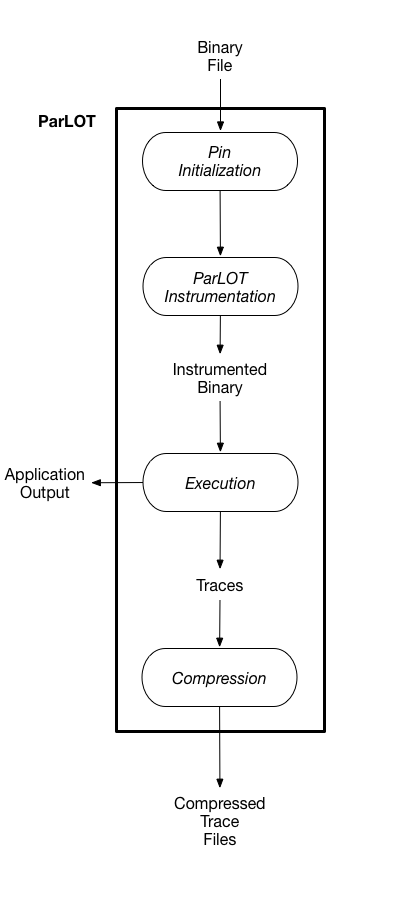
\includegraphics[width=2in]{overview.png}
\caption{ Overview of \parlot}
\label{overview}
\end{figure}
